%!TEX root = ../Thesis.tex
%Chapter 6

\chapter{Rectification in a minimal model}
\label{Chapter6}
\lhead{Chapter 6. \emph{Rectification in a minimal model}} % Write in your own chapter title to set the page header
%
In this chapter we present a minimalistic model system which shows rectification. It is composed of two unequal atoms subjected to linear forces and in contact with effective Langevin baths
induced by optical molasses. Analytic expressions of the heat currents in the steady state and the rectification coefficient are spelled out. Asymmetric heat transport is found in this linear system if both the bath temperatures and the temperature dependent bath-system couplings are exchanged. The model can be realized with two ions  in  either common or individual traps. This physical setting allows for a natural temperature dependence of the coupling to the baths.
We also explore the parameter space of the model to optimize asymmetric heat current and find
conditions for maximal rectification. High rectification corresponds to a good match of the power spectra of the ions for forward temperature bias and mismatch  for reverse bias, which may be understood by the behavior of dissipative normal modes.
%
\newpage
%
\section{Introduction \label{sec:Introduction}}

As previously discussed in the introduction to this part of the thesis, the presence of thermal rectification in the first models was explained by the temperature dependences of the phonon bands (power spectra) of the different segments of the chain \cite{Terraneo2002,Li2004}. This temperature dependence of the phonon bands brings two different extreme situations. The phonon spectra of neighboring parts of the chain match, meaning they overlap significantly, which implies a good transfer of energy. Conversely, if the spectra of the neighboring parts mismatch, meaning they do not overlap significantly, there will be a bad thermal conduction. If the spectra of the parts of the chain are affected differently by the temperature, then the magnitude of the net heat current will change with the sign of the applied temperature bias. Temperature dependence of the phonon bands occurs naturally in systems where there are non-linear (anharmonic) interactions, therefore non-linearities have been regarded recurrently as an essential element for rectification \cite{Li2012,Li2008,Hu2006,Zeng2008,Segal2005,Segal2005b,Katz2016,Benenti2016}. However, it was later pointed out by Pereira \cite{Pereira2017} that anharmonicity is not a necessary condition for rectification. Rectification can also take place in harmonic systems where there is some structural asymmetry and temperature-dependence of the system parameters.

In this chapter we put forward a minimalistic model for rectification composed of two neighboring atoms of different mass interacting harmonically and in contact with thermal baths with temperature dependent coupling. The model admits a  natural realization in terms of two trapped ions subjected to  Doppler cooling lasers, which provide the
necessary temperature dependence of the coupling parameters. Apart from the possibility of a physical realization, another interesting
feature is the analytical treatment, which facilitates greatly the exploration in parameter  space to  identify regimes of maximal rectification. The explicit solution of the stationary regime also provides tools for a better understanding of the physics and enhanced control. For example the match or mismatch of the spectra of the two masses for forward and reverse bias configurations, which will be made evident for the parameters with maximal
rectification, may be analyzed in terms of dissipative normal modes characterized by complex eigenvalues.

The model may be compared and related to other simple models. The localization of the
structural asymmetry in a  small spatial region, by a ``defect'', ``impurity'', or asymmetrical molecule has been proposed e.g. in
several anharmonic models \cite{Segal2005b,Pons2017,Alexander2020}.
Segal and Nitzan proposed models with some similarities to ours \cite{Segal2005,Segal2005b}, specifically an anharmonic chain
with different couplings to both baths. They also worked out  quantum models \cite{Segal2005,Segal2005b} in terms of an N-level
system asymmetrically coupled to the baths. Both types of models have ``harmonic limits'', which in the chain is reached by making the potentials
harmonic, and in the quantum one by taking $N$ to infinity assuming equispaced levels.
The asymmetrical couplings however, were not interchanged when reversing the temperature bias
(in these models that interchange would have suppressed the asymmetry because the forward bias configuration becomes a mirror image of the reverse bias one), so that
the harmonic limit did not give any rectification.

The chapter is organized as follows: In Section \ref{sec:Physical_Model}
we describe the physical model and its dynamical equations. In Section \ref{sec:covMatrix} we introduce the  covariance matrix and  derive the equation  that it satisfies in the steady state. In Section \ref{sec:solutions} we solve the covariance matrix equation and find analytical expressions for the steady-state temperatures of the masses and heat currents. In Section \ref{sec:TrappedIonSetUp} we relate the parameters of the model to those of Doppler cooled trapped ions. In Section \ref{sec:lookingForR} we look for configurations with high rectification. We also study the power spectra of the oscillators, which confirm the match or mismatch pattern for rectification. Finally, in Section \ref{sec:Conclusions} we summarize the results and present the conclusions.

\begin{figure}
  \center
  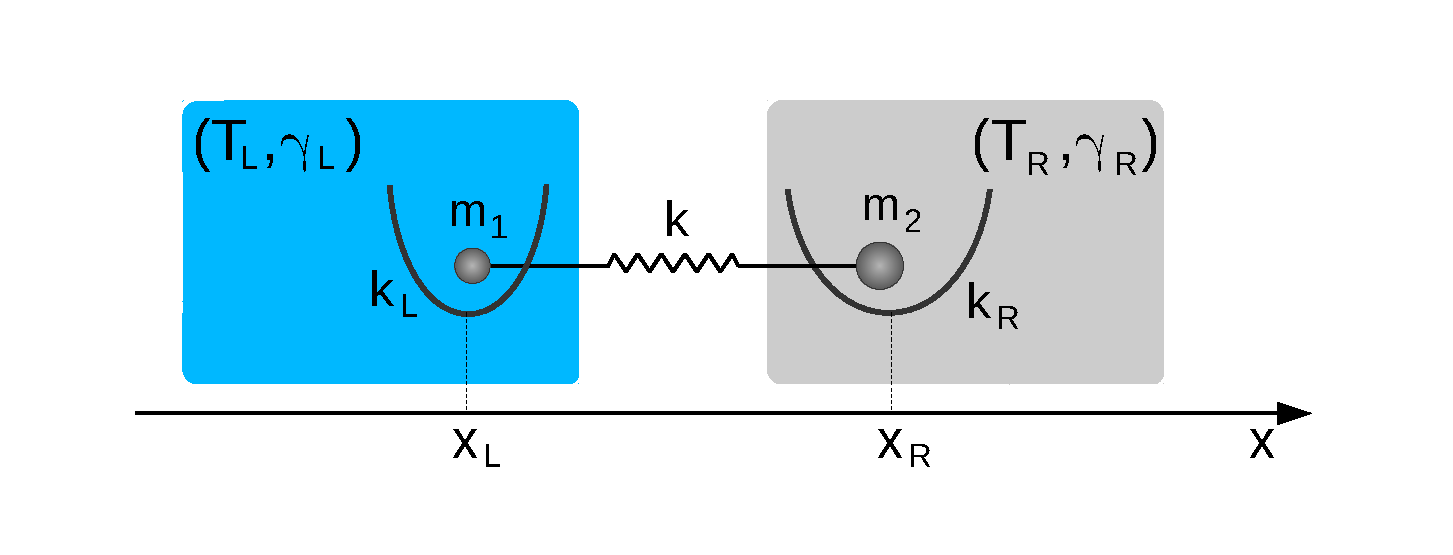
\includegraphics[width=0.75\linewidth]{Figures/model_diagram.pdf}
  \caption{Diagram of the model described in Section \ref{sec:Physical_Model}. Two masses are coupled to each other through a spring constant $k$. Each mass is harmonically trapped and connected to a bath characterized by its temperature $T_i$ and its friction coefficient $\gamma_i$. }
  \label{fig:model_diagram}
\end{figure}
%
%
%
%
\section{Physical Model \label{sec:Physical_Model}}
%
%
%
%
The physical model consists of two masses $m_1$ and $m_2$ coupled to each other by a harmonic interaction with spring constant $k$ and natural length $x_e$. The masses $m_1$ and $m_2$ are confined by  harmonic potentials centered at $x_L$, $x_R$ with spring constants $k_L$, $k_R$  respectively (see Fig. \ref{fig:model_diagram}). The Hamiltonian describing this model is
%
\begin{equation}
  H = \frac{p_1^2}{2m_1} + \frac{p_2^2}{2m_2} + V(x_1,x_2),
  \label{eq:chapter6_HamiltonianOriginalCordinates}
\end{equation}
%
with $V(x_1,x_2)=\frac{k}{2}\left( x_1 - x_2 - x_e \right)^2 + \frac{k_L}{2}\left( x_1 - x_L \right)^2 + \frac{k_R}{2}\left( x_2 - x_R \right)^2$,  where $\{x_i,p_i\}_{i=1,2}$ are the position and momentum of each mass. Switching from the original coordinates $x_i$ to displacements with respect to the equilibrium positions of the system $q_i = x_i - x_i^{eq}$, where $x_i^{eq}$ are the solutions to $\partial_{x_i}V(x_1,x_2)=0$, the Hamiltonian can be written as
%
\begin{align}
  H &= \frac{p_1^2}{2m_1} + \frac{p_2^2}{2m_2} + \frac{k+k_L}{2}q_1^2\nonumber\\ &+ \frac{k+k_R}{2}q_2^2 - k q_1 q_2 + V(x_1^{eq},x_2^{eq}).
  \label{eq:chapter6_Hamiltonian}
\end{align}
%
Dropping the constant term, this has the form of  the Hamiltonian of a system around a stable equilibrium point,
%
\begin{equation}
  H = \frac{1}{2} \overrightarrow{p}^\mathsf{T}\mathbb{M}^{-1}\overrightarrow{p} + \frac{1}{2} \overrightarrow{q}^\mathsf{T}\mathbb{K}\overrightarrow{q},
\label{generic}
\end{equation}
%
where $\overrightarrow{q} = \left(q_1,q_2\right)^\mathsf{T}$, $\overrightarrow{p} = \left(p_1,p_2\right)^\mathsf{T}$, $\mathbb{M} = diag(m_1,m_2)$ is the mass matrix of the system and $\mathbb{K}$ is the Hessian matrix of the potential at the equilibrium point, i.e., $\mathbb{K}_{ij} = \partial^2_{x_i,x_j}V(\overrightarrow{x})\Big|_{\overrightarrow{x} = \overrightarrow{x}^{eq}}$. In this model  $\mathbb{K}_{11} = k + k_L$, $\mathbb{K}_{22} = k + k_R$ and $\mathbb{K}_{12} = \mathbb{K}_{21} = -k$.
We shall see later that
the generic form (\ref{generic}) can be adapted to different physical settings, in particular to
two ions in individual traps, or to two ions in a common trap.

The  masses are in contact with Langevin baths, which will be denoted as $L$ (for left) and $R$ (for right), at temperatures $T_{L}$ and $T_R$ for  the mass $m_1$ and $m_2$ respectively (see Fig. \ref{fig:model_diagram}). The equations of motion of the system, taking into account the Hamiltonian and the Langevin baths are
%
\begin{align}
  \dot{q}_1 &= \frac{p_1}{m_1},\;\;\;\;
  \dot{q}_2 = \frac{p_2}{m_2},\nonumber
  \\
  \dot{p}_1 &= -(k+k_L)q_1 + k q_2 -\frac{\gamma_L}{m_1} p_1 + \xi_L(t),\nonumber
  \\
  \dot{p}_2 &= -(k+k_R)q_2 + k q_1 -\frac{\gamma_R}{m_2} p_2 + \xi_R(t),
\end{align}
%
where $\gamma_L$, $\gamma_R$ are the friction coefficients of the baths and $\xi_L(t)$, $\xi_R(t)$ are Gaussian white-noise-like forces. The Gaussian forces have zero mean over noise realizations ($\expval{ \xi_L(t) } = \expval{ \xi_R(t) } = 0 $) and satisfy the correlations $\expval{ \xi_L(t)\xi_R(t') } = 0$, $\expval{ \xi_L(t)\xi_L(t') } = 2D_L\delta(t-t')$, $\expval{ \xi_R(t)\xi_R(t') } = 2D_R\delta(t-t')$. $D_L$ and $D_R$ are the diffusion coefficients, which satisfy the fluctuation-dissipation theorem, $D_L = \gamma_L k_B T_L$, $D_R =\gamma_R k_B T_R$, where  $k_B$ is the Boltzmann constant.

It is useful to define the phase-space vector $\overrightarrow{r}(t) = \left( \overrightarrow{q}, \mathbb{M}^{-1}\overrightarrow{p} \right)^\mathsf{T}$ (note that $\overrightarrow{v} = \mathbb{M}^{-1}\overrightarrow{p}$ is just the velocity vector).  The equations of motion are
%
\begin{equation}
  \dot{\overrightarrow{r}}(t) = \mathbb{A} \, \overrightarrow{r}(t) + \mathbb{L}\overrightarrow{\xi}(t),
  \label{eq:chapter6_vectorEqOfMotion}
\end{equation}
%
with
%
\begin{align}
  \mathbb{A} &=
  \left(
  \begin{array}{cc}
    \mathbb{0}_{2 \times 2} & \mathbb{1}_{2 \times 2}
    \\
    -\mathbb{M}^{-1}\mathbb{K} & -\mathbb{M}^{-1}\bbGamma
  \end{array}
  \right),
  \nonumber
  \\
  \mathbb{L} &=
  \left(
  \begin{array}{c}
    \mathbb{0}_{2\times 2} \\ \mathbb{M}^{-1}
  \end{array}
  \right),
  \label{eq:chapter6_Dynamical_Matrix}
\end{align}
%
and $\overrightarrow{\xi}(t) = \left( \xi_L(t),\xi_R(t) \right)^\mathsf{T}$, $\bbGamma = diag(\gamma_L,\gamma_R)$. $\mathbb{0}_{n\times n}$ and $\mathbb{1}_{n\times n}$ are the $n$-dimensional squared 0 matrix and identity matrix respectively. With the vector notation the correlation of the white-noise forces can be written as
%
\begin{equation}
  \expval{\overrightarrow{\xi}(t)\overrightarrow{\xi}(t')^\mathsf{T}} = 2 \mathbb{D}\delta(t-t'),
\end{equation}
%
where $\mathbb{D} = diag(D_L,D_R)$.
%
%
%
%
%
%
\section{Covariance matrix in the steady state\label{sec:covMatrix}}
%
%
%
%
%
%
In order to look for the steady state currents in the system we will make use of the covariance matrix $\mathbb{C}(t)$ which is defined as
%
\begin{equation}
\mathbb{C}(t) = \expval{\overrightarrow{r}(t)\overrightarrow{r}(t)^\mathsf{T}}.
\end{equation}
%
The relation between the kinetic temperatures of the masses, $T_1(t)$ and  $T_2(t)$, and the covariance matrix is given by
%
\begin{align}
  T_1(t) &\equiv \frac{\expval{ p_1^2(t)}}{m_1 k_B} = \frac{m_1 C_{3,3}(t)}{k_B},
  \nonumber\\
   T_2(t) &\equiv \frac{\expval{ p_2^2(t)}}{m_2 k_B} = \frac{m_2 C_{4,4}(t)}{k_B}.
  \label{eq:chapter6_Temperature_definition}
\end{align}
%
As discussed in section \ref{sec:chapter5_steadyState}, the covariances of the positions and velocities of the masses could be calculated integrating eq. \eqref{eq:chapter6_vectorEqOfMotion} over an ensemble of noise realizations $\overrightarrow{\xi}(t)$ and taking the corresponding expectation values in the steady state. However, in section \ref{sec:chapter5_steadyState} we also pointed out the tremendous cost of doing this, so we introduced a way to linearize the system that let us find the steady-state covariances as the solutions for a set of algebraic equations \cite{Sarkka2019,Rieder1967,Casher1971}. In this case the system dynamics are already linear, so we can directly use the steady-state method described in \ref{sec:chapter5_steadyState}. Besides, the solutions of the steady-state equations will be analytical for this two oscillators model.

To begin, we differentiate $\mathbb{C}(t)$ with respect to time and use Eq. \eqref{eq:chapter6_vectorEqOfMotion} to get
%
\begin{align}
  \frac{d}{dt}\mathbb{C}(t) &=
  \mathbb{A}\mathbb{C}(t) +
  \mathbb{C}(t) \mathbb{A}^\mathsf{T}
  \nonumber\\
  &+
  \mathbb{L}\expval{ \overrightarrow{\xi}(t)\overrightarrow{r}(t)^\mathsf{T}}
  %\nonumber\\
 % &+
+
  \expval{ \overrightarrow{r}(t)\overrightarrow{\xi}(t)^\mathsf{T}}\mathbb{L}^\mathsf{T}.
  \label{eq:chapter6_evolutionOfCovariances}
\end{align}
%
The solution of Eq. \eqref{eq:chapter6_evolutionOfCovariances} can be used to find the kinetic temperatures of the masses at all times but we are only interested in the steady-state values, \textit{i.e.} the asymptotic values for $t\to \infty$. In the steady state, the covariance matrix is constant ($\frac{d}{dt}\mathbb{C}(t)=0$), therefore it satisfies
%
\begin{equation}
  \mathbb{A}\mathbb{C}^{s.s.} +
  \mathbb{C}^{s.s.} \mathbb{A}^\mathsf{T}=
  - \mathbb{L}\expval{ \overrightarrow{\xi}\overrightarrow{r}^\mathsf{T}}^{s.s.}
  - \expval{ \overrightarrow{r}\overrightarrow{\xi}^\mathsf{T}}^{s.s.}\mathbb{L}^\mathsf{T},
  \label{eq:chapter6_SteadyStateEquationToyModel_raw}
\end{equation}
%
with $\small\{\cdot\small\}^{s.s.}\equiv \lim\limits_{t \to \infty} \small\{\cdot\small\}(t)$. The two terms $\expval{ \overrightarrow{\xi}\overrightarrow{r}^\mathsf{T}}^{s.s.}$ and  $\expval{\overrightarrow{r}\overrightarrow{\xi}^\mathsf{T}}^{s.s.}$ in \eqref{eq:chapter6_SteadyStateEquationToyModel_raw} can be calculated using Novikov's theorem \cite{Novikov1965} as explained in section \ref{sec:chapter5_HeatFlow}. We get
%
\begin{equation}
  \expval{ \overrightarrow{\xi}(t)\overrightarrow{r}(t)^\mathsf{T}} = \mathbb{D}\mathbb{L}^\mathsf{T}.
\end{equation}
%
We have therefore, the following algebraic equation for the steady-state covariance matrix
%
\begin{equation}
  \mathbb{A}\mathbb{C}^{s.s.} +
  \mathbb{C}^{s.s.}\mathbb{A}^\mathsf{T}
  =
  -\mathbb{B},
  \label{eq:chapter6_SteadyStateEquationToyModel}
\end{equation}
%
with $\mathbb{B} = 2 \mathbb{L}\mathbb{D}\mathbb{L}^\mathsf{T}$. By definition, the covariance matrix is  symmetric, but there are also  additional restrictions imposed by the equations of motion and the steady-state condition, which reduce the dimensionality of the problem of solving Eq. \eqref{eq:chapter6_SteadyStateEquationToyModel} \cite{Simon2019}. Since ${d \expval{ q_i q_j }}/{dt} = 0$ in the steady state, we have
%
\begin{align}
  \expval{ p_1 q_1}^{s.s.} &= \expval{ p_2 q_2}^{s.s.} = 0,\nonumber\\
  \frac{\expval{ p_1 q_2}^{s.s.}}{m_1}&=-\frac{\expval{ q_1 p_2}^{s.s.}}{m_2}.
  \label{eq:chapter6_ExtraConditionSteadyState}
\end{align}
%
Taking \eqref{eq:chapter6_ExtraConditionSteadyState} into account, the steady-state covariance matrix takes the form
%
\begin{equation}
  \begin{split}
    \mathbb{C}^{s.s.} =
    \left(
    \begin{array}{cccc}
      \expval{ q_1^2}^{s.s.}  & \expval{ q_1 q_2}^{s.s.}  & 0 & \frac{\expval{ p_2 q_1}^{s.s.} }{m_2} \\
      \expval{ q_1 q_2}^{s.s.}  & \expval{ q_2^2}^{s.s.}  & -\frac{\expval{ p_2 q_1}^{s.s.} }{m_2} & 0 \\
      0 & -\frac{\expval{ p_2 q_1}^{s.s.} }{m_2} & \frac{\expval{ p_1^2}^{s.s.} }{m_1^2} & \frac{\expval{ p_1 p_2}^{s.s.} }{m_1 m_2} \\
      \frac{\expval{ p_2 q_1}^{s.s.} }{m_2} & 0 & \frac{\expval{ p_1 p_2}^{s.s.} }{m_1 m_2} & \frac{\expval{ p_2^2}^{s.s.} }{m_2^2} \\
      \end{array}
      \right)
    \end{split}
    \label{eq:chapter6_steadyStateCovarianceMatrix}\,.
\end{equation}
%
The explicit set of equations for the components of $\mathbb{C}^{s.s}$ can be found in Appendix \ref{Appendix:SteadyStateEquations}.
%
%
%
%
%
\section{Solutions\label{sec:solutions}}
%
%
%
%

%
In this section we use the solution to Eq. \eqref{eq:chapter6_SteadyStateEquationToyModel} to write down the temperatures and currents in the steady state. We use {\it Mathematica} to find analytic expressions for the temperatures,
%
\begin{align}
  T_1 &= \frac{T_L \mathcal{P}_{1,L}(k) + T_R \mathcal{P}_{1,R}(k)}{\mathcal{D}(k)},\nonumber
  %
  \\
  %
  T_2 &= \frac{T_L \mathcal{P}_{2,L}(k) + T_R \mathcal{P}_{2,R}(k)}{\mathcal{D}(k)},
  %
  \label{eq:chapter6_ModelBTemperatures}
\end{align}
%
where $\mathcal{D}(k) =  \sum\limits_{n=0}^2 \mathcal{D}_n k^n$ and $\mathcal{P}_{i,(L/R)}(k) = \sum\limits_{n=0}^2 a_{i,n,(L/R)} k^n$ are polynomials in the coupling constant $k$ with coefficients
%

%\begin{widetext}
  \begin{align}
    \mathcal{D}_0 &= a_{1,0,L} = a_{2,0,R}
    \nonumber\\
    & = \gamma _L \gamma _R\! \left[h^{(1)}\! \left(\gamma_L k_R +\gamma_R k_L \right)+\left(m_1 k_R-m_2 k_L\right)^2\right]\!,
    \nonumber\\
    %
    \mathcal{D}_1 &= a_{1,1,L} = a_{2,1,R}
    \nonumber\\
    &= \gamma _L \gamma _R\! \left[h^{(0)} h^{(1)}\!+2 \left(m_1-m_2\right) \left(m_1 k_R-m_2 k_L\right)\right]\!,
    %
    \nonumber\\
    %
    \mathcal{D}_2 &= h^{(0)} h^{(2)},\nonumber
    %
    \\
    %
    a_{1,2,L} &= \gamma _L \left(m_2 h^{(1)} + \gamma_R (m_1 - m_2)^2 \right),\nonumber
    %
    \\
    %
    a_{1,2,R} &= h^{(1)} m_1 \gamma_R,\nonumber
    %
    \\
    %
    a_{2,2,L} &= h^{(1)} m_2 \gamma_L,\nonumber
    %
    \\
    %
    a_{2,2,R} &= \gamma _R \left( m_1 h^{(1)} + \gamma_L (m_1-m_2)^2 \right),\nonumber
    %
    \\
    %
    a_{1,0,R} &= a_{1,1,R} = a_{2,0,L} = a_{2,1,L} = 0,
    %
    \label{eq:chapter6_SolutionPolynomialCoefficients}
  \end{align}
%\end{widetext}
%
where
%
\begin{equation}
h^{(n)}\equiv \gamma_R m_1^n + \gamma_L m_2^n.
\end{equation}
%
The currents from the baths to the masses are given by eq. \eqref{eq:chapter5_BathHeatFlowNovikov}
%
\begin{equation}
    J_L = k_B \frac{\gamma_L}{m_1} \left( T_L - T_1 \right),\;\;\;
    J_R = k_B \frac{\gamma_R}{m_2} \left( T_R - T_2 \right),
    \label{eq:chapter6_currents_definition}
\end{equation}
\\
%
with $T_i$ given by Eq. \eqref{eq:chapter6_ModelBTemperatures}. Since, in the steady state, $J_L = -J_R$ we will use the shorthand notation $J \equiv J_L$. Substituting Eq. \eqref{eq:chapter6_ModelBTemperatures} into Eq.  \eqref{eq:chapter6_currents_definition} we get for the heat current
%
\begin{equation}
  J = \kappa\;(T_L - T_R),
  \label{eq:chapter6_CurrentsInModelB}
\end{equation}
%
where $\kappa = k_B {k^2\gamma_L \gamma_R h^{(1)}}/{\mathcal{D}(k)}$ acts as an effective thermal conductance.
%
%
%
%
\section{Relation of the Model to a trapped ion setup \label{sec:TrappedIonSetUp}}
%
In this section we discuss the realization of the model with  a pair of trapped ions. We consider two different setups: two ions in a collective trap, and two ions in individual traps. Later in Section \ref{sec:lookingForR} we shall focus on two ions in individual traps to illustrate the analysis of rectification.

In both setups we assume strong confinement in the radial direction, making the effective dynamics one-dimensional. We will also assume that the confinement in the axial direction is purely electrostatic, which makes the effective spring constant independent of the mass of the ions \cite{Leibfried2003}. Additionally, we will relate the temperatures and friction coefficients of the Langevin baths to those corresponding to Doppler cooling.
%
%
\subsection{Collective trap}
%
%
Consider two ions of unit charge with masses $m_1$ and $m_2$ trapped in a collective trap. Assuming strong radial confinement and purely electrostatic axial confinement, both ions feel the same harmonic oscillator potential with trapping constant $k_{trap}$ \cite{Leibfried2003}. The potential describing the system is
%
\begin{equation}
  V_{collective} = \frac{1}{2}k_{trap} \left( x_1^2 + x_2^2\right) + \frac{\mathcal{C}}{x_2-x_1},
\end{equation}
%
with $\mathcal{C}={Q^2}/({4\pi\varepsilon_0})$. The equilibrium positions for this potential are
%
\begin{equation}
  x_2^{eq} = -x_1^{eq} =
  \label{eq:chapter6_equilibriumPositionsCollectiveTrap}\left(\frac{1}{2}\right)^{2/3} \left(\frac{Q^2}{4\pi\varepsilon_0 k_{trap}}\right)^{1/3}.
\end{equation}
%
Assuming small oscillations of the ions around the equilibrium positions, the Hessian matrix of the system is
%
\begin{align}
  \mathbb{K}_{1,2} &= -\frac{Q^2}{2\pi\varepsilon_0}\frac{1}{(x_2^{eq}-x_1^{eq})^3} = -k_{trap},\nonumber
  \\
  \mathbb{K}_{1,1} &= k_{trap} + \frac{Q^2}{2\pi\varepsilon_0}\frac{1}{(x_2^{eq}-x_1^{eq})^3} = 2 k_{trap},\nonumber
  \\
  \mathbb{K}_{2,2} &= k_{trap} + \frac{Q^2}{2\pi\varepsilon_0}\frac{1}{(x_2^{eq}-x_1^{eq})^3} = 2 k_{trap}.
  \label{eq:chapter6_HessianOffDiagonalCollective}
\end{align}
%
Using Eq. \eqref{eq:chapter6_HessianOffDiagonalCollective} we can relate the parameters of this physical setup to those of the model described in Section \ref{sec:Physical_Model},
%
\begin{equation}
  k_L = k_R = k = k_{trap}.
\end{equation}
%
%
%
\subsection{Individual on-site traps}
%
%
%
We can make the same assumptions for the axial confinement as in the previous subsection but now each of the ions is in an individual trap with spring constants $k_{trap,L}$ and $k_{trap,R}$ respectively. The potential of the system is
%
\begin{align}
    V_{individual} &= \frac{1}{2}k_{trap,L}\left(x_1 -x_L\right)^2 +\frac{1}{2}k_{trap, R}\left(x_2 -x_R\right)^2 \nonumber \\&+ \frac{\mathcal{C}}{x_2-x_1},
\end{align}
%
where $x_L$ and $x_R$ are the center positions of the on-site traps. The elements of the Hessian matrix in the equilibrium position are
%
\begin{align}
  \mathbb{K}_{1,2} &= -\frac{Q^2}{2\pi\varepsilon_0}\frac{1}{(x_2^{eq}-x_1^{eq})^3},\nonumber
  \\
  \mathbb{K}_{1,1} &= k_{trap,L} + \frac{Q^2}{2\pi\varepsilon_0}\frac{1}{(x_2^{eq}-x_1^{eq})^3},\nonumber
  \\
  \mathbb{K}_{2,2} &= k_{trap,R} + \frac{Q^2}{2\pi\varepsilon_0}\frac{1}{(x_2^{eq}-x_1^{eq})^3}.
  \label{eq:chapter6_HessianOffDiagonalOnSite}
\end{align}
%
Comparing the parameters in Eq. \eqref{eq:chapter6_HessianOffDiagonalOnSite} with those in the model described in Section \ref{sec:Physical_Model} we identify
\begin{align}
  k_L &= k_{trap,L},\nonumber\\
  k_R &= k_{trap,R},\nonumber\\
  k &= \frac{Q^2}{2\pi\varepsilon_0}\frac{1}{(x_2^{eq}-x_1^{eq})^3}\,.
\end{align}
%
In this case, the analytic expressions for the equilibrium positions are more complicated. We get for the distance between the equilibrium positions of the ions
%
\begin{align}
  &(x_2 - x_1)^{(eq)} = \frac{1}{3} \Delta x_{LR}\nonumber\\
  &- \frac{1}{6}\Big[ \frac{2^{2/3}\zeta}{k_{trap,L} k_{trap,R} (k_{trap,L} + k_{trap,R})}\nonumber\\
  &+ \frac{2^{4/3} k_{trap,L} k_{trap,R} (k_{trap,L} + k_{trap,R}) (x_R-x_L)^2}{\zeta} \Big]\,,
\end{align}
%
where $\Delta x_{LR} = (x_R-x_L)$ and $\zeta = \left( Y - \eta \right)^{(1/3)}$, with
%
\begin{eqnarray}
&&Y = 3 \sqrt{3} \bigg\{\mathcal{C} k_{trap,L}^4 k_{trap,R}^4 \left(k_{trap,L}+k_{trap,R}\right)^{7}
\nonumber\\
&&\times\left[4 k_{trap,L} k_{trap,R} \Delta x_{LR}^3+27 \mathcal{C} \left(k_{trap,L}+k_{trap,R}\!\right)\!\right]\!\!\bigg\}^{\!1/2}\!,
\nonumber
%
\\
  %%
&&\eta =  k_{trap,L}^2 k_{trap,R}^2 \left(k_{trap,L}+k_{trap,R}\right)^{3}
\nonumber\\
&&\times\left[2 k_{trap,L} k_{trap,R} \Delta x_{LR}^3+27 \mathcal{C} \left(k_{trap,L}+k_{trap,R}\right)\right]\!.
\end{eqnarray}
%
In this setup, the coupling between the ions $k$ can be controlled by changing the distance between the on-site traps.
%
%
%
\subsection{Optical molasses and Langevin baths}
%
%
%
As discussed in section \ref{sec:chapter5_PhysicalSystem}, the Langevin dynamics can be implemented in a trapped-ion setup with the technique of optical molasses \cite{Chu1985,Cohen1992,Metcalf1999,Metcalf2003}. The damping-like force in the Langevin equation comes from the absorption of the photons by the ions, while the diffusive force ($\overrightarrow{\xi}(t)$) is originated by the random recoil of the ions when they emit photons. To recall what was explained in \ref{sec:chapter5_PhysicalSystem}, the effect of the optical molass amounts to having an effective temperature $T_{molass}$ and effective friction coefficient $\gamma_{molass}$ which are controlled with the laser intensity $I$ and frequency detuning $\delta$ with respect to the selected internal atomic transition. The following expressions describe the molass effect \cite{Cohen1992,Metcalf2003,Ruiz2014}
%
\begin{align}
  \gamma_{molass}(I,\delta) &= -4 \hbar \left(\frac{\delta + \omega_0}{c}\right)^2 \left(\frac{I}{I_0}\right)\frac{2\delta/\Gamma}{\left[1 + (2\delta/\Gamma)^2\right]^2},\nonumber\\
  %
  T_{molass}(\delta) &= -\frac{\hbar \Gamma}{4 k_B} \frac{1+(2\delta/\Gamma)^2}{(2\delta/\Gamma)},
  \label{eq:chapter6_DopplerCoolingToyModel}
\end{align}
%
where $\omega_0$ is the frequency of the selected internal atomic transition of the ion, $\Gamma$ is the natural width (decay rate) of the excited state, and $I_0$ is the saturation intensity. For fixed $\Gamma$ and $I$, $\gamma_{molass}$ depends on $\delta$, and thus, indirectly, on the temperature $T_{molass}$.
%
%
%
\section{Looking for rectification\label{sec:lookingForR}}
%
%
%
%First let us define what we exactly mean by \textit{rectification}.
There is rectification if the flux $J$  for the forward temperature bias is different from the flux $\tilde{J}$ for reverse bias
with the baths exchanged.  To measure rectification, we will use the rectification coefficient $0\le R\le 1$ defined as
%
\begin{equation}
  R \equiv \frac{\abs{|J|-|\tilde{J}|}}{\max(|J|,|\tilde{J}|)}
  = 1 - \min{ \left( \frac{\kappa}{\tilde{\kappa}} , \frac{\tilde{\kappa}}{\kappa} \right) },
  \label{eq:chapter6_Rectification}
\end{equation}
%
where $\kappa$, $\tilde{\kappa}$ are the heat conductance in the forward and reversed (after the baths are exchanged) configurations. The important point here is to define what is meant by \textit{exchanging the baths}. We consider that a bath is characterized, not only by its temperature $T$ but also by its coupling  to the system by means of the friction coefficient $\gamma$, so, exchanging the baths is achieved by exchanging both the temperatures and the friction coefficients, as summarized in Table \ref{tab:reversed_bath}. For generic models this
choice is a matter of definition, but for trapped ions it is a natural way to proceed.

When implementing temperatures and friction coefficients by lasers according to
%, this exchange operation is performed by changing the values of the intensities and detunings acting on each ion (
Eq. \eqref{eq:chapter6_DopplerCoolingToyModel}, the exchange operation is straightforward when the two ions are either of the same species or isotopes of each other, since the only required action to exchange temperatures is to exchange the detunings without modifying the intensities. The detuning exchange in turn automatically exchanges the friction coefficients. However, for two different species, which involve two different atomic transitions, the laser wavelengths and the decay rates $\Gamma$ depend on the species. Then, exchanging the temperatures by modifying the detunings, keeping the laser intensities constant, does not necessarily imply an exchange of the friction coefficients. Nevertheless it is possible to adjust the laser intensities so that the friction coefficients get exchanged and that is the assumption hereafter. In terms of the analysis of rectification in Ref. \cite{Pereira2017}, we are adding a temperature dependent feature to the system, namely,  the friction coefficients depend on the bath temperature
and are exchanged as the baths are reversed.

\begin{figure}
  \center
  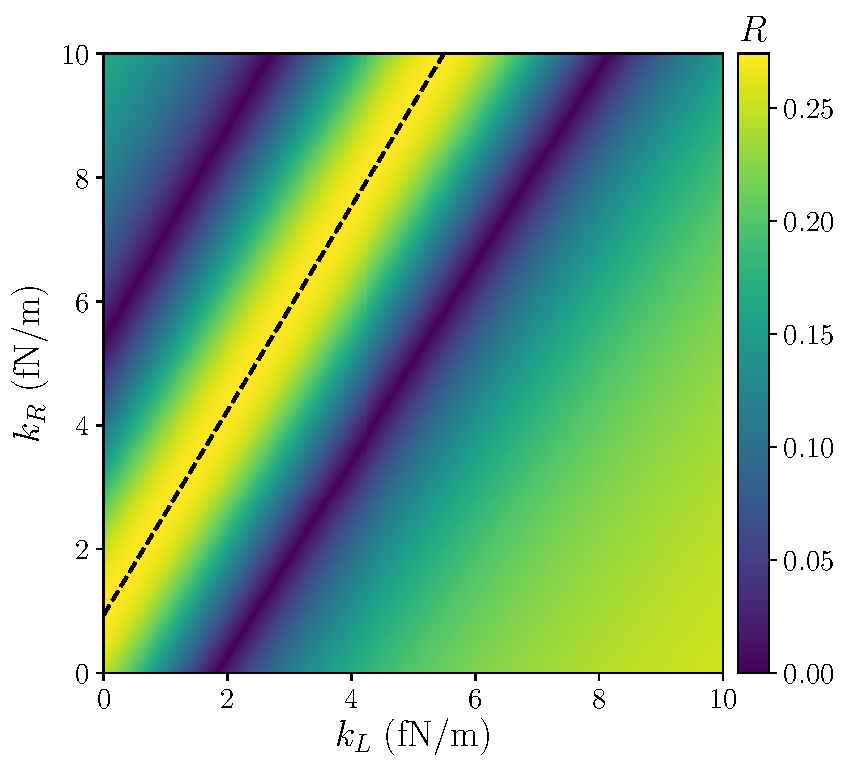
\includegraphics[width=0.75\linewidth]{Figures/RwMPlota.pdf}
  \caption{Rectification, $R$, in the $k_L k_R$ plane for $k = 1.17$ fN/m, $\gamma_L = 6.75\times 10^{-22}$ kg/s, and $\gamma_R = 4.64\gamma_L$, $m_1 = 24.305$ a.u., $m_2 = 40.078$ a.u. The dashed  line represents Eq.  (\ref{eq:chapter6_MaxRLines}).}
  \label{fig:Fig_rectification_K_plane}
\end{figure}


%that is, the ratio between the difference of heat currents and the largest one. As defined, $R=0$ for no asymmetry of the heat currents and $R=1$ when they are maximally asymmetric.

\begin{table}[]
\center
\caption{Definition of forward and reversed (exchanged) bath configurations. The variables with a tilde are the ones for the ``reversed'' configuration.}
\begin{tabular}{lcc}
\hline
& forward                & reversed                                                       \\ \hline
Bath Friction    & $\gamma_L$, $\gamma_R$ & $\tilde{\gamma}_L =\gamma_R $,  $\tilde{\gamma}_R =\gamma_L $   \\
Bath Temperature & $T_L$, $T_R$           & $\tilde{T}_L =T_R $,  $\tilde{T}_R =T_L $                     \\
\hline
\end{tabular}
\label{tab:reversed_bath}
\end{table}
%
%
\subsection{Parametric exploration}
%
%
%
We have explored thoroughly the space formed by the parameters of the model $m_1,m_2,k,k_L,k_R,\gamma_L,\gamma_R$, to find
and maximize asymmetric heat transport. We have fixed the values of some of the parameters to realistic ones while varying the rest. Unless stated otherwise the masses are
$m_1 = 24.305$ a.u. and $m_2 = 40.078$ a.u., which correspond to Mg and Ca, whose ions are broadly used in trapped-ion physics. According to eqs. \eqref{eq:chapter6_CurrentsInModelB} and \eqref{eq:chapter6_Rectification} does not formally depend on the bath temperatures in this model for given friction coefficients. Of course the friction coefficients depend on the temperature indirectly, but also on laser intensities, see Eq. \eqref{eq:chapter6_DopplerCoolingToyModel}, so in the parametric space $m_1,m_2,k,k_L,k_R,\gamma_L,\gamma_R$ there is no need to specify the bath temperatures to analyze the rectification in the following. The bath temperatures will be needed though to calculate the power spectra, and play an implicit role in the central assumption that their exchange implies an exchange of friction coefficients.

Figure \ref{fig:Fig_rectification_K_plane} depicts the values of the rectification after sweeping the $k_L k_R$ plane for fixed values of $k$, $\gamma_L$, and $\gamma_R$. There is a ridge in the $k_L,k_R$ plane for which the rectification is maximal. $\partial_{k_L}R = 0$ may be
solved explicitly but the solution is too long to be displayed here. In a weak dissipation regime
(${\gamma_L}/{m_1}<<\sqrt{{k}/{m_1}}$, ${\gamma_R}/{m_2}<<\sqrt{{k}/{m_2}}$), a Taylor series around $(\gamma_L,\gamma_R) = (0,0)$ gives in zeroth order
%.i.e., ${\gamma_L}/{m_1}<<\sqrt{{k}/{m_1}}$, ${\gamma_R}/{m_2}<<\sqrt{{k}/{m_2}}$, the ridge is given approximately by
a straight line for the ridge,
%
\begin{equation}
  \frac{k+k_R}{m_2} = \frac{k+k_L}{m_1}.
  \label{eq:chapter6_MaxRLines}
\end{equation}
%
Eq. \eqref{eq:chapter6_MaxRLines} implies the resonance condition $\omega_L = \omega_R$
for the effective oscillation frequencies $\omega_L = \sqrt{{(k+k_L)}/{m_1}}$ and $\omega_R = \sqrt{{(k+k_R)}/{m_2}}$,
see Eq. (\ref{eq:chapter6_Hamiltonian}). The lowest order correction to  Eq. \eqref{eq:chapter6_MaxRLines} implies a small shift of the line,
keeping the same slope,
%
\begin{equation}
  \frac{k+k_R}{m_2} = \frac{k+k_L}{m_1} + \frac{(m_2\gamma_L+m_1\gamma_R)(m_1\gamma_L+m_2\gamma_R)}{2m_1m_2(m_2^2-m_1^2)}.
  \label{eq:chapter6_MaxRLines_correction}
\end{equation}
%
In a trapped-ion context the condition \eqref{eq:chapter6_MaxRLines} may be imposed by adjusting the distance of the traps for fixed $k_L$ and $k_R$. Besides the line of maximum rectification, Fig. \ref{fig:Fig_rectification_K_plane} also shows two lines where rectification is zero.
At these lines forward and backward fluxes cross.
%, The lines correspond to the boundaries in which the heat conductance for the reversed configuration surpasses the forward configuration. Inside of these boundaries heat propagates easily for a forward bias ($T_L>T_R$), whereas the opposite happens outside. In Fig. \ref{fig:Fig_rectification_K_plane}, the lines of zero rectification look parallel to the one of maximum rectification. This is however only a limiting behavior for weak dissipation.
Solving $R=0$ with a Taylor series around $(\gamma_L,\gamma_R) = (0,0)$ gives, up to second order in friction coefficients,  the two approximate solutions
%
\begin{align}
k_R &= k_L\left[\frac{m_2}{m_1}\pm\frac{1}{2k}\sqrt{\frac{m_2\gamma_L\gamma_R^3}{m_1^3}}\right]
\nonumber\\
&+k\left[\frac{m_2}{m_1}\left(1\pm \frac{ 2 m_1 m_2 \gamma_R + (m_1^2 + m_2^2)\gamma_L }{2\sqrt{m_1 m_2^3 \gamma_L \gamma_R}} \right)-1\right]
\nonumber\\
&\pm\frac{1}{2}\sqrt{\frac{m_2\gamma_L\gamma_R^3}{m_1^3}} + \gamma_R\frac{(m_1^2+m_2^2)\gamma_L + m_1m_2\gamma_R}{2m_1^2(m_2-m_1)}.
\label{eq:chapter6_zeroRlines}
\end{align}
%
The term $\pm\frac{1}{2k}\sqrt{{m_2\gamma_L\gamma_R^3}/{m_1^3}}$ in Eq. \eqref{eq:chapter6_zeroRlines} makes the slopes of the
two zero-rectification lines different from each other and also from the maximum-rectification line. This difference is however
hardly noticeable for weak dissipation as in  Fig. \ref{fig:Fig_rectification_K_plane}.

Interestingly, along the maximum line  \eqref{eq:chapter6_MaxRLines} the rectification no longer depends on the spring constants of the model,
see  Eqs. \eqref{eq:chapter6_CurrentsInModelB}  and \eqref{eq:chapter6_Rectification},
%
\begin{equation}
    R=
    \begin{cases}
      1-\frac{a+g}{1+ag} &\text{ if }a>1,g>1\text{ or }a<1,g<1\\
      1-\frac{1+ag}{a+g} &\text{ if }a>1,g<1\text{ or }a<1,g>1,
    \end{cases}
  \label{eq:chapter6_maxRExpression}
\end{equation}
%
it only depends on the mass and friction coefficient ratios $a$ and $g$
%
\begin{align}
  a = m_2/m_1,\;\;\;\;
  g = \gamma_R/\gamma_L.
\end{align}
%
%The maximal rectification found does not scale with the magnitude of the masses or the friction coefficients, just with their ratios.
Besides a high value of $R$, it is desirable to have a significant current $J_{max}$
%when a forward temperature bias is applied to the rectifier
%, as in some cases an increase of $R$ is accompanied by an overall decrease of the heat currents
\cite{Simon2019}. Using again  Eq. \eqref{eq:chapter6_MaxRLines} in the expression for the currents \eqref{eq:chapter6_CurrentsInModelB}, the maximum current $J_{\max} = \max(\big|{J}\big|,\big|\tilde{J}\big|)$ is
%
\begin{align}
    &J_{\max}=\begin{cases}
   \frac{k_B g\gamma_L k^2 \abs{T_L-T_R}}{(a+g)(g\gamma_L^2(k_L+k)+k^2m_1)} &
   \text{ if }\begin{cases}a>1,g>1\\
   \text{ or }a<1,g<1\end{cases}
    \\
    \frac{k_B g\gamma_L k^2 \abs{T_L-T_R}}{(1+ag)(g\gamma_L^2(k_L+k)+k^2m_1)}&\text{ if }
    \begin{cases}a>1,g<1
    \\\text{ or }a<1,g>1\end{cases}
    \end{cases}
    \label{eq:chapter6_maxJExpression}
\end{align}
%
Now we analyze how the parameters $a$ and $g$ affect the maximum current $J_{max}$ in \eqref{eq:chapter6_maxJExpression}. To do this, we can divide the $ag$ plane in four quadrants by the axes $a = 1$ and $g = 1$ (in those axes $R = 0$). In Eq. \eqref{eq:chapter6_maxJExpression} the parameter $a$ appears only in the denominator, thus for a higher $a$, a smaller current is found. The quadrants with $a < 1$ will be better for achieving large currents. $g$ appears both in the numerator and denominator so there is no obvious advantageous quadrant for this parameter.

Equation \eqref{eq:chapter6_maxRExpression} is symmetric upon the transformations $a \leftrightarrow 1/a$ and $g \leftrightarrow 1/g$. Using a logarithmic scale for $a$ and $g$, the resulting $R$ map is symmetric with respect to the $a=1$ and $g=1$ axes. We can thus limit ourselves to analyze the quadrant $a > 1$, $g > 1$.


\begin{figure}
  \center
  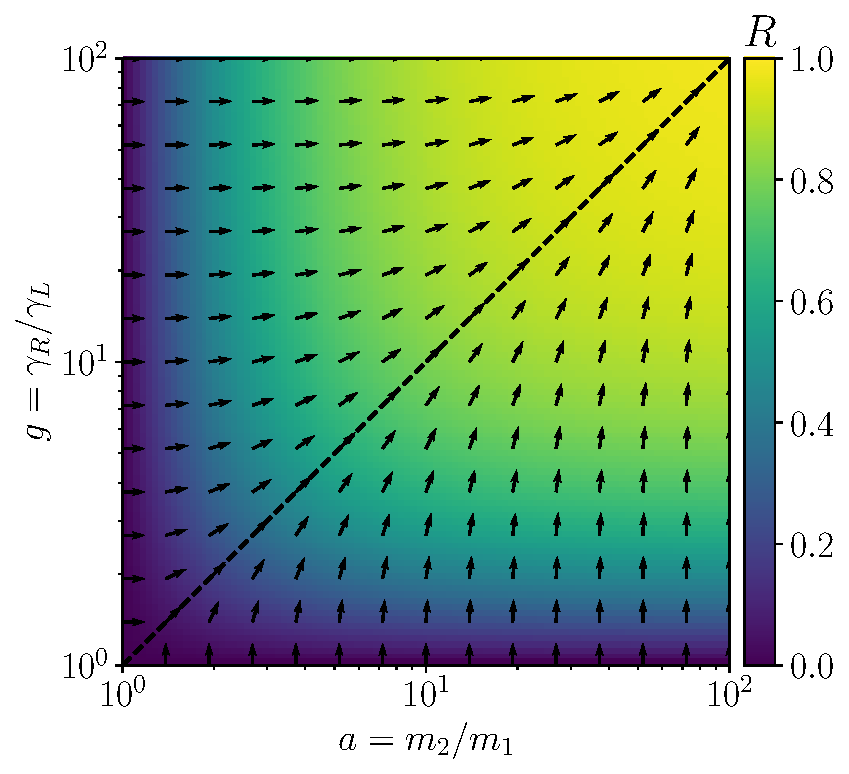
\includegraphics[width=0.75\linewidth]{Figures/Rade.pdf}
  \caption{Rectification factor, $R$, given by Eq. \eqref{eq:chapter6_maxRExpression}.}
  \label{fig:R_g_a_plane}
\end{figure}

Figure \ref{fig:R_g_a_plane} shows the rectification given by Eq. \eqref{eq:chapter6_maxRExpression} in terms of $a$ and $g$. If one follows the direction of the gradient vector of R, $\overrightarrow{\nabla}R\equiv\left( \partial_a R, \partial_g R \right)$, which is indicated in fig. \ref{fig:R_g_a_plane} by the black arrows, it becomes clear that the fastest way of increasing $R$ is following the diagonal dashed line of $a=g$. Therefore we decided to vary $a$ and $g$ following a common value $c=a = g$. The effect of varying  the common value $c$ may be seen in Fig. \ref{fig:Fig_PerfectRectification}, which  shows the rectification in Eq. \eqref{eq:chapter6_maxRExpression}. $R$ tends to one for large $c$.
%
%
\subsection{Spectral match/mismatch approach to rectification}
%
%
%
\begin{figure}
  \center
  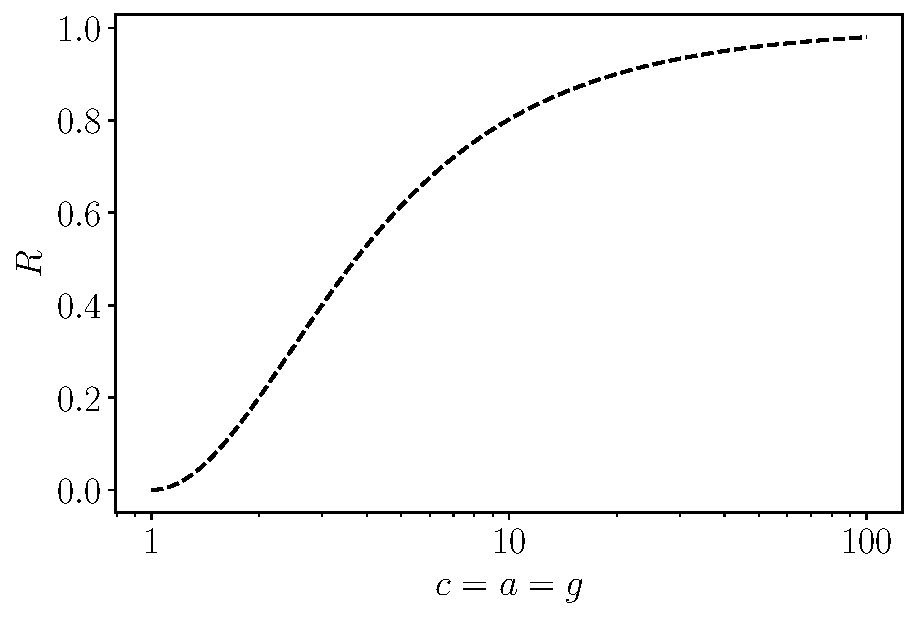
\includegraphics[width=0.75\linewidth]{Figures/CC.pdf}
  \caption{Rectification for different values of $c=m_2/m_1=\gamma_R/\gamma_L$ when the maximum condition in the $k_L k_R$ plane is satisfied (Eq. \eqref{eq:chapter6_MaxRLines}).}
  \label{fig:Fig_PerfectRectification}
\end{figure}

If there is a good match between the phonon spectra of the ions (i.e., their peaks overlap in a broad range of frequencies) for a certain baths configuration, and mismatch when the baths exchange, the system will present heat rectification \cite{Terraneo2002,Li2004}.
We have studied the spectra of the ions in our model for several sets of parameters exhibiting no rectification or strong rectification. The spectra are calculated  through the spectral density matrix. For a real-valued stochastic process $\overrightarrow{x}(t)$, its spectral density matrix is defined as \cite{Sarkka2019}
%
\begin{equation}
  \mathbb{S}_{\overrightarrow{x}}(\omega) \equiv \expval{ \overrightarrow{X}(\omega) \overrightarrow{X}^\mathsf{T}(-\omega) },
  \label{eq:chapter6_SpectralDensityDefinition}
\end{equation}
%
with $\overrightarrow{X}(\omega)$ being the Fourier transform of $\overrightarrow{x}(t)$ (we use the convention of factors of $1$ and ${1}/{(2\pi)}$ for the transform and the inverse transform). A justification of the use of the spectral density matrix to understand heat transport arises from the Wiener-Khinchin theorem \cite{Sarkka2019}, which says that the correlation matrix of a stationary stochastic process in the steady state is the inverse Fourier transform of its spectral density matrix $\expval{\overrightarrow{r}(t)\overrightarrow{r}^\mathsf{T}(t+\tau)} = \mathcal{F}^{-1}[\mathbb{S}_{\overrightarrow{r}}(\omega)](\tau)$. Thus  the covariance matrix in the steady state is
%
\begin{equation}
  \mathbb{C}^{s.s.} = \frac{1}{2\pi} \int_{-\infty}^{\infty}d\omega\;\mathbb{S}_{\overrightarrow{r}}(\omega).
  \label{eq:chapter6_Wiener-Khinchin}
\end{equation}
%
Eq. \eqref{eq:chapter6_Wiener-Khinchin} directly connects the spectral density matrix to the steady-state temperature
since  $T_1^{s.s.} = {m_1 C_{3,3}^{s.s.}}/{k_B}$ and $T_2^{s.s.} = {m_2 C_{4,4}^{s.s.}}/{k_B}$, and, therefore, to the heat currents,
see  Eqs.(\ref{eq:chapter6_Temperature_definition}) and (\ref{eq:chapter6_currents_definition}).


\begin{figure}[t]
  \center
  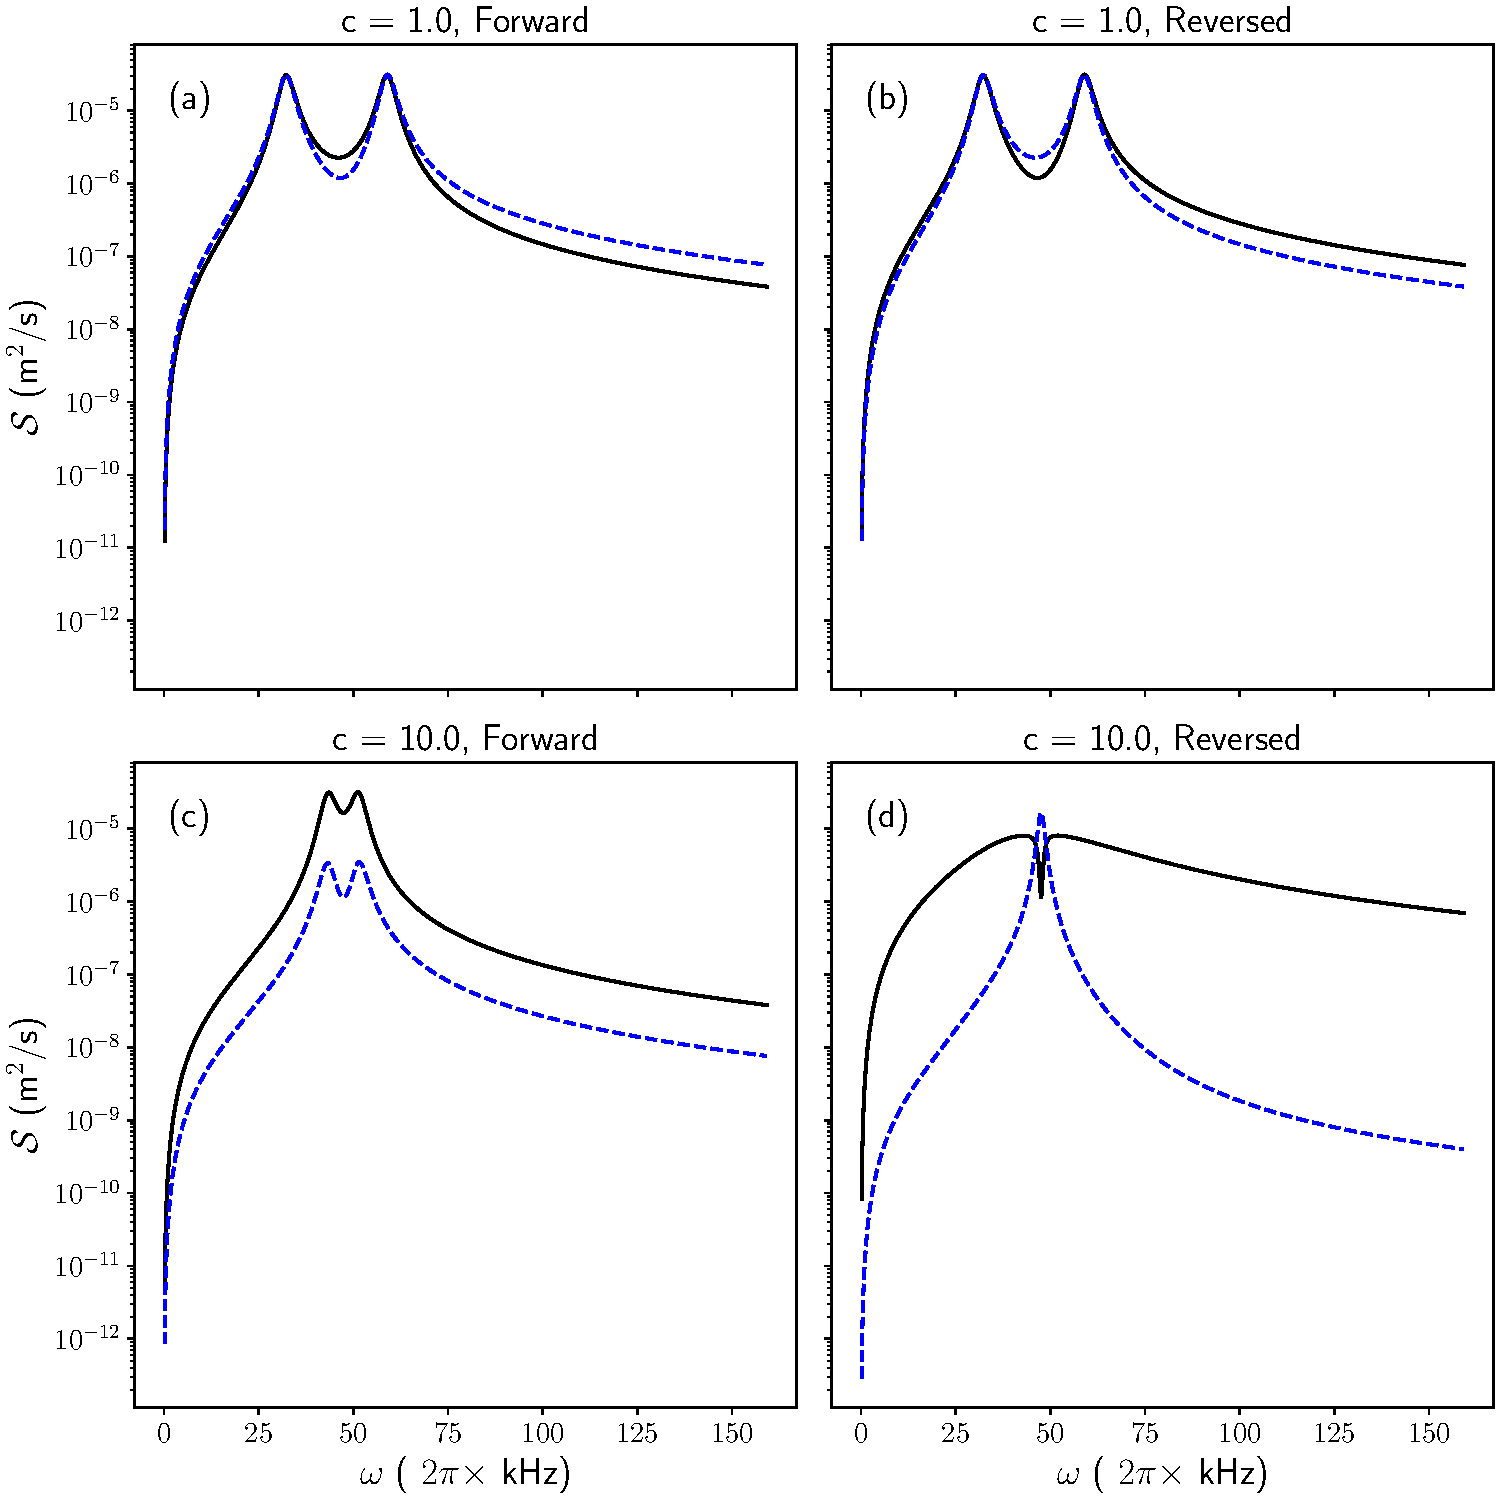
\includegraphics[width=0.75\linewidth]{Figures/SpectrumComparative.pdf}
  \caption{Spectral densities of the velocities of the ions ($r_3$ and $r_4$) corresponding to $T_L=\tilde{T}_R=2$ mK, $T_R=\tilde{T}_L=1$ mK, and  two values of $c$ in Fig. \ref{fig:Fig_PerfectRectification}: (a), (b) for $c=1$ and (c), (d) for $c=10$. Solid, black lines are for the left ion spectral density ${\cal{S}}_1(\omega)$ and dashed, blue lines for the right ion spectral density
 ${\cal{S}}_2(\omega)$. Dot-dashed, vertical lines mark the frequencies of the normal modes of the system. The spectra are multiplied by their corresponding masses so that  the areas are proportional to the steady-state temperatures, see  Eq. \eqref{eq:chapter6_Wiener-Khinchin}. (a) and (b) correspond to $R = 0$:  the overlap between the phonon bands is the same in forward and reversed configurations. (c) and (d) correspond to $R\approx 0.8$:  in the forward configuration (c)  the phonons match better than in the reversed configuration (d).}
  \label{fig:Figure_Spectra}
\end{figure}

The Fourier transform of the vector process $\overrightarrow{r}(t)$ describing the evolution of our system, see Eq. (\ref{eq:chapter6_vectorEqOfMotion}),
is $\overrightarrow{R}(\omega) = \left( i \omega - \mathbb{A} \right)^{-1}\mathbb{L}\overrightarrow{\Xi}(\omega)$ with $\overrightarrow{\Xi}(\omega)$ being the Fourier transform of the white noise $\overrightarrow{\xi}(t)$. Note that $\overrightarrow{\Xi}(\omega)$ is not square-integrable, however its spectral density is $\mathbb{S}_{\overrightarrow{\xi}}(\omega) = 2 \mathbb{D}$ \cite{Sarkka2019}, which is flat as expected for a white noise. Therefore, the spectral density matrix of the system is
%
\begin{equation}
  \mathbb{S}_{\overrightarrow{r}} (\omega)= 2 \left(  \mathbb{A} - i\omega\right)^{-1}\mathbb{L}\mathbb{D}\mathbb{L}^\mathsf{T}\left(  \mathbb{A} + i\omega\right)^{-\mathsf{T}}.
  \label{eq:chapter6_SpectralDensityToyModelB}
\end{equation}
%
%As we can see in Eq. \eqref{eq:chapter6_SpectralDensityToyModelB},
The imaginary part of the eigenvalues of the dynamical matrix $\mathbb{A}$ correspond to the peaks in the spectrum whereas the real part dictates their width. Eq. \eqref{eq:chapter6_SpectralDensityToyModelB} gives after direct computation
%
\begin{equation}
  \mathbb{S}_{\overrightarrow{r}}(\omega) = 2 k_B \frac{\gamma_L T_L\mathbb{S}_L(i\omega)+\gamma_L T_R\mathbb{S}_R(i\omega)}{(m_1 m_2)^2 P_\mathbb{A}(i\omega)P_\mathbb{A}(-i\omega)},
\end{equation}
%
where $P_\mathbb{A}(\lambda)$ is the characteristic polynomial of the dynamical matrix $\mathbb{A}$ and $\mathbb{S}_L(\omega)$, $\mathbb{S}_R(\omega)$ are the matrix polynomials in the angular frequency $\omega$ whose coefficients are defined in Appendix \ref{Appendix:SpectralDensity}. We give
%Equation \eqref{eq:chapter6_SpectralDensitiesVelocities} gives the full expressions of
the spectral densities for the velocities, ${\cal{S}}_1\equiv\mathbb{S}_{3,3}(\omega) = \expval{R_3(\omega)R_3(-\omega)}$ for the left ion, and ${\cal S}_2\equiv\mathbb{S}_{4,4}(\omega) = \expval{R_4(\omega)R_4(-\omega)}$ for the right ion, since they are the elements related to the calculation of the heat current using Eq. \eqref{eq:chapter6_Wiener-Khinchin},
%
  \begin{align}
    {\cal S}_1(\omega) &= 2 k_B \frac{\gamma_R k^2 T_R \omega ^2+\gamma_L T_L \left[\omega ^4 \left(\gamma_R^2-2 k m_2-2 k_R m_2\right)+\omega ^2 (k+k_R)^2+m_2^2 \omega ^6\right]}{(m_1 m_2)^2 P_\mathbb{A}(i\omega)P_\mathbb{A}(-i\omega)},\nonumber\\
    %
%    \nonumber\\
    %
%    \mathbb{S}_{4,4}(\omega)
{\cal S}_2(\omega)
&= 2 k_B \frac{\gamma_L k^2 T_L \omega ^2+\gamma_R T_R \left[\omega ^4 \left(\gamma_L^2-2 k m_1-2 k_L m_1\right)+\omega ^2 (k+k_L)^2+m_1^2 \omega ^6\right]}{(m_1 m_2)^2 P_\mathbb{A}(i\omega)P_\mathbb{A}(-i\omega)}.
    \label{eq:chapter6_SpectralDensitiesVelocities}
  \end{align}
%
%The spectral densities of the masses depend explicitly on the temperatures on the baths, as well as implicitly through the dependence of the friction coefficients if the laser cooling baths are used.
Figure \ref{fig:Figure_Spectra} depicts a series of plots of the spectra given by Eq. \eqref{eq:chapter6_SpectralDensitiesVelocities}, corresponding to two points in Fig. \ref{fig:Fig_PerfectRectification}. (The calculation for the reverse bias is done with the substitutions in Table \ref{tab:reversed_bath}.)
For $c=1$ (Fig. \ref{fig:Figure_Spectra}(a) and (b)) there is no rectification, since the spectra match in the forward (a) and reversed (b) configurations. However, for $c=10$ (Fig. \ref{fig:Figure_Spectra}(c) and (d), $R\approx 0.8$) the picture is very different: there is a good match between the spectra in the forward configuration but not for the reversed configuration. It is interesting to analyze how the system changes from $c=1$ to $c=10$ (see fig. \ref{fig:Figure_Eigenvals_NormalModes})using the dissipative normal modes of the system, which may be found by diagonalizing the dynamical matrix $\mathbb{A}$, Eq. \eqref{eq:chapter6_Dynamical_Matrix}. The frequencies of the peaks in Fig. \ref{fig:Figure_Spectra} are given by the imaginary part of the eigenvalues $\lambda_\mathbb{A} = \lambda_r + i \lambda_i$ of $\mathbb{A}$. Likewise, the width depends on  the real part of the eigenvalues. For the forward configuration, the normal frequencies (position of the peaks) come closer to each other as $c$ is increased, while the widths remain practically constant. To understand why the real part remains practically constant, we recall that we have chosen to work with spring constants that satisfy Eq. \eqref{eq:chapter6_MaxRLines} and making the mass and friction coefficient ratios equal to $c$, \textit{i.e.}, $ c\equiv m_2/m_1 = \gamma_R/\gamma_L$. The (dissipative) terms in $\mathbb{A}$ responsible for the real parts in the eigenvalues are,
for the forward configuration,  $\gamma_L/m_1$ and $\gamma_R/m_2 = (c \gamma_L)/(c m_1) = \gamma_L/m_1$, which are constant for every value of $c$. On the contrary, in the reverse bias configuration  the dissipative terms in the dynamical matrix  are $\tilde{\gamma}_L/m_1 = \gamma_R/m_1 = c\gamma_L/m_1$ and $\tilde{\gamma}_R/m_2 = \gamma_L/ (c m_1)$, with opposite behavior with respect to $c$. The real parts of the eigenvalues
also behave quite differently for reverse bias, one of them gets closer to the imaginary axis for $c=10$,
see Fig. \ref{fig:Figure_Spectra} (d), where this mode  concerns mostly the right ion,
the only one excited at the peak frequency, while the other eigenvalue  moves far from the imaginary axis so a peak is not noticeable
at the imaginary value (left dotted-dashed line) any more.

\begin{figure}
  \center
  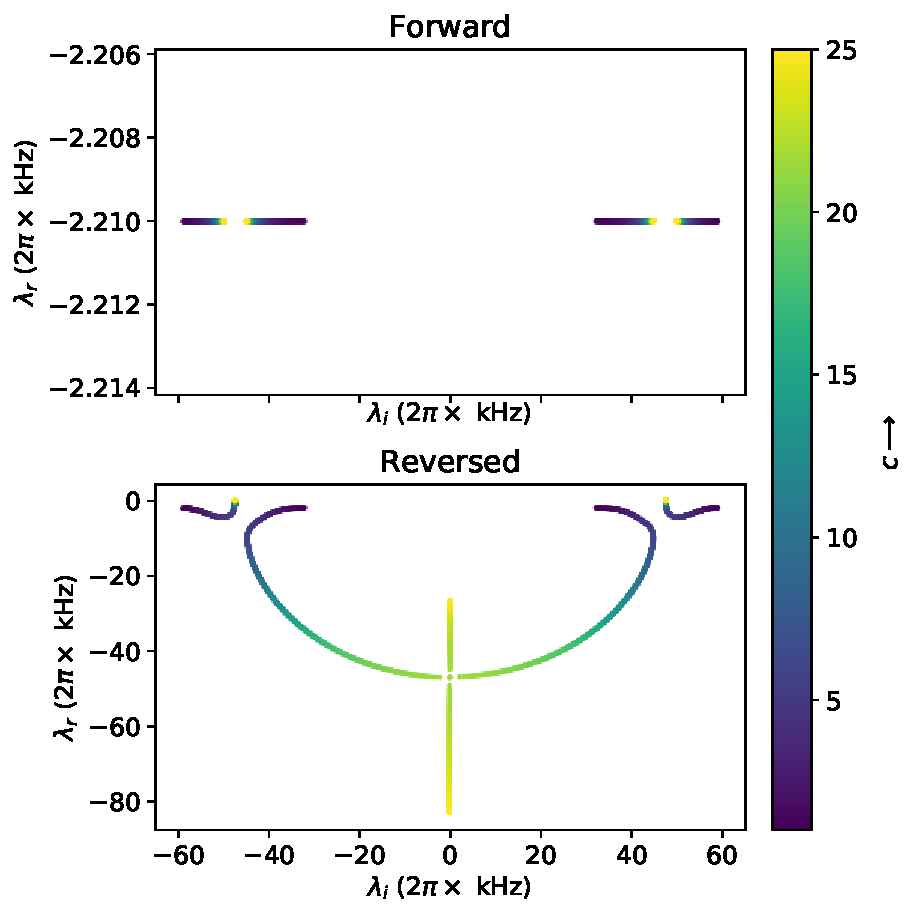
\includegraphics[width=0.75\linewidth]{Figures/Eigenvals_NormalModes.pdf}
  \caption{The evolution of the dissipative normal modes of the system as the asymmetry parameter $c$ increases is shown in this plot. $\lambda_r$, $\lambda_i$ stand for the real and imaginary parts of the eigenvectors of the dynamical matrix $\mathbb{A}$.}
  \label{fig:Figure_Eigenvals_NormalModes}
\end{figure}


%
\section{Conclusions \label{sec:Conclusions}}
%
We have studied heat rectification in a model composed of two coupled harmonic oscillators connected to Langevin baths, which could be realized with trapped ions and optical molasses. This simple model allows analytical treatment but still has enough complexity to examine different ingredients that can produce rectification. %We have also derived analytical expressions for the heat currents and local temperatures.
Our results demonstrate in a simple but realistic model that harmonic systems can rectificate heat current if they have features which depend on the temperature  \cite{Pereira2017}. We implement this notion of temperature-dependent features by defining the baths exchange operation as an exchange of both temperatures and coupling parameters of the baths to the system. The temperature dependence of the bath-system coupling  occurs naturally in laser-cooled trapped ion setups.

We have also studied the phonon spectra of the system, aided by a normal mode analysis,
comparing the match/mismatch of the phonon bands, to reach the conclusion that the band match/mismatch description for heat rectification is also valid for systems which are purely harmonic, as long as there are temperature-dependent features.
We hope this chapter sheds more light into the topic of heat rectification and that encourages more research regarding its physical implementation on chains of trapped ions.
